\chapter{Conservatiebiologie}\label{ch:b3:conservation-biology}

In 1813 zag Audubon drie dagen lang een zwerm trekduiven over Kentucky
trekken die de hemel verduisterde; er waren er misschien vijf miljard,
een kwart van alle vogels van Noord-Amerika. Op 1~september 1914 stierf
de laatste, een vrouwtje dat Martha heette, in de dierentuin van
Cincinnati. De soort was niet zeldzaam toen haar achteruitgang begon;
zij werd bij treinladingen geoogst, haar bossen werden gekapt, en een
vogel die alleen in geweldige kolonies broedde kon niet meer broeden
zodra de kolonies waren uitgedund onder een omvang die niemand heeft
gemeten. In 1995 was de kakapo, een nachtelijke papegaai van
Nieuw-Zeeland die niet kan vliegen, teruggelopen tot eenenvijftig
vogels; elk daarvan heeft sindsdien een naam gekregen, is gewogen, van
een zender voorzien en op het juiste ogenblik een extra maaltijd
aangeboden, en er zijn er nu tweehonderdvijftig. In datzelfde jaar
werden eenendertig grijze wolven in Yellowstone uitgezet, zeventig jaar
nadat de laatste inheemse roedel was doodgeschoten; binnen twee
decennia waren de wapiti's verhuisd, waren de wilgen langs de rivieren
teruggekeerd, en de bevers met hen. De conservatiebiologie past de
populatiegenetica, de ecologie en het gedrag uit dit boek toe op één
praktische vraag --- hoe soorten van verdwijnen te weerhouden --- en
haar rekenkunde is de rekenkunde van kleine getallen.

\section{Waarom kleine populaties sterven}

\begin{definition}[De risico's van kleinheid]\label{def:b3:conservation-biology:small}
\index{demografische toevalligheid}\index{toevalligheid van de omgeving}\index{Allee-effect}\index{uitstervingsdraaikolk}\index{minimaal levensvatbare populatie}
Een grote populatie loopt terug wanneer haar sterftecijfer haar
geboortecijfer overtreft; een kleine kan verdwijnen zonder dat een van
beide verandert. \emph{Demografische toevalligheid} is de kans dat er
onder een handvol individuen toevallig meer sterven dan er worden
geboren, of dat alle overlevenden mannelijk zijn: zij telt onder een
paar dozijn. \emph{Toevalligheid van de omgeving} --- een slechte
winter, een droogte, een ziekte --- treft elk individu tegelijk, en een
populatie van een paar honderd die een grote zou uitzitten kan worden
weggevaagd; \emph{rampen} vormen de staart daarvan. Het
\emph{Allee-effect} laat het groeitempo per hoofd bij lage dichtheid
dalen --- partners zijn niet te vinden, koloniebroeders kunnen niet
nestelen, kudden kunnen hun jongen niet verdedigen, de zwermen van de
trekduif konden de roofdieren die hun jongen namen niet meer verzadigen
--- zodat de populatie onder een drempeldichtheid uit zichzelf naar nul
loopt. En onder een paar honderd verlagen de genetische processen van
de volgende paragraaf de fitness van generatie op generatie. Die voeden
elkaar: een kleinere populatie verliest variatie, wordt minder
vruchtbaar, wordt kleiner, wordt eerder door toeval getroffen en
verliest nog meer --- de \emph{uitstervingsdraaikolk} (Gilpin en Soulé,
1986). Een \emph{minimaal levensvatbare populatie} is de omvang
waarboven de kans op uitsterven binnen een genoemde termijn (zeg
\qty{5}{\%} in een eeuw) aanvaardbaar is; zij hangt af van de biologie
van de soort en van hoe wisselvallig haar omgeving is, en ligt
gewoonlijk in de duizenden.
\end{definition}

\begin{omfigure}
\begin{tikzpicture}[every node/.style={font=\scriptsize}, >=stealth]
  \node[draw, thick, rounded corners, fill=omThm!20, align=center] (small) at (0,0) {populatie\\wordt klein};
  \node[draw, thick, rounded corners, fill=omDef!20, align=center] (drift) at (3.4,1.6) {drift en inteelt:\\variatie weg, $F$ stijgt};
  \node[draw, thick, rounded corners, fill=omDef!20, align=center] (fit) at (6.8,0) {fitness daalt:\\minder jongen, meer ziekte};
  \node[draw, thick, rounded corners, fill=omDef!20, align=center] (chance) at (3.4,-1.6) {demografisch toeval en dat van\\de omgeving bijten harder};
  \node[draw, thick, rounded corners, fill=omProp!25, align=center] (allee) at (9.9,0) {Allee-effect:\\groeitempo negatief};
  \draw[->, very thick] (small) -- (drift); \draw[->, very thick] (drift) -- (fit); \draw[->, very thick] (fit) -- (chance); \draw[->, very thick] (chance) -- (small);
  \draw[->, thick, omProp!80!black] (fit) -- (allee); \draw[->, thick, omProp!80!black] (allee.south) .. controls (9.9,-3) and (0,-3.4) .. (small.south);
  \node[align=center, font=\tiny] at (3.4,0) {de uitstervingsdraaikolk:\\elke ronde doet de populatie\\krimpen en versnelt de volgende};
  \node[left, align=right, font=\tiny] at (-1.7,1.5) {verlies van leefgebied, oogst,\\uitheemse roofdieren, ziekte\\duwen de populatie erin};
  \draw[->, thick, gray] (-1.6,1.2) -- (small.north west);
\end{tikzpicture}

{\small De \omterm{def:b3:conservation-biology:small}{uitstervingsdraaikolk}. Een klap van buiten maakt een
populatie klein; de kleinheid verliest dan variatie, verlaagt de
fitness, stelt de populatie aan het toeval bloot en maakt haar nog
kleiner. De taak van het natuurbehoud is de lus te breken voordat zij
zich sluit.}
\end{omfigure}

\begin{theorem}[Effectieve populatiegrootte]\label{thm:b3:conservation-biology:ne}
\index{effectieve populatiegrootte}\index{geslachtsverhouding}\index{harmonisch gemiddelde}\index{inteeltcoëfficiënt}\index{heterozygotie}
Het tempo waarmee een populatie variatie verliest en inteelt opbouwt
wordt niet bepaald door haar tellingsgrootte $N$ maar door haar
\emph{effectieve grootte} $N_{e}$: de omvang van een ideale populatie
--- constant, willekeurig parend, met gelijke \omterm{thm:b3:conservation-biology:ne}{geslachtsverhouding} en
Poisson-verdeelde gezinsgrootten --- die met hetzelfde tempo
heterozygotie zou verliezen. Drie afwijkingen van het ideaal verlagen
haar. Een ongelijke \omterm{thm:b3:conservation-biology:ne}{geslachtsverhouding}, met $N_{m}$ broedende
mannetjes en $N_{f}$ vrouwtjes:
\[
N_{e} = \frac{4N_{m}N_{f}}{N_{m} + N_{f}} ;
\]
één mannetje en honderd vrouwtjes geven $N_{e} \approx 4$. Een
schommelende omvang over $t$ generaties: $N_{e}$ is het
\emph{harmonische gemiddelde} van de generatiegrootten,
$1/N_{e} = (1/t)\sum 1/N_{i}$, dat door de kleinste wordt beheerst ---
een populatie van duizend die ooit door tien is gegaan heeft over dat
bestek een $N_{e}$ nabij honderd. En een variantie in de gezinsgrootte
boven Poisson verlaagt haar nog verder. In een populatie met effectieve
grootte $N_{e}$ stijgt de \emph{\omterm{thm:b3:conservation-biology:ne}{inteeltcoëfficiënt}} $F$ --- de kans dat
de twee allelen op een locus in een individu kopieën zijn van één
voorouderlijk allel --- met $1/2N_{e}$ per generatie,
\[
F_{t} = 1 - \Bigl(1 - \frac{1}{2N_{e}}\Bigr)^{t} \approx \frac{t}{2N_{e}},
\qquad H_{t} = H_{0}\Bigl(1 - \frac{1}{2N_{e}}\Bigr)^{t} ,
\]
en de \emph{heterozygotie} $H$ dooft met hetzelfde tempo uit. De
vuistregel van Franklin, ``50/500'': $N_{e} \ge 50$ houdt de inteelt
onder \qty{1}{\%} per generatie, het tempo dat dierfokkers verdragen;
$N_{e} \ge
500$ laat de mutatie de variatie vervangen die de drift wegneemt. Omdat
$N_{e}$ gewoonlijk een tiende van de tellingsgrootte is, vraagt de
regel om populaties van vijfhonderd tot vijfduizend.
\end{theorem}
\begin{proof}
Twee willekeurig uit de populatie getrokken gameten zijn in de ideale
populatie met kans $1/2N$ kopieën van hetzelfde ouderlijke allel, en
dat is de aanwas van $F$; de heterozygotie is $1 - F$ geschaald, dus
vermenigvuldigt elke generatie haar met $(1 - 1/2N_{e})$, wat het
exponentiële verval geeft en, voor $t \ll N_{e}$, de lineaire stijging
van $F$. \omterm{thm:b3:conservation-biology:ne}{Geslachtsverhouding}: de helft van de genen komt van elk
geslacht, dus is de kans dat twee gameten een ouderlijk allel delen
$\tfrac{1}{4}\cdot\tfrac{1}{2N_{m}} +
\tfrac{1}{4}\cdot\tfrac{1}{2N_{f}}$ (een kwart van de paren is beide
van vaderskant, een kwart beide van moederskant); dat gelijkstellen aan
$1/2N_{e}$ geeft $1/N_{e} = 1/(4N_{m}) + 1/(4N_{f})$, de formule.
Schommeling: de heterozygotie na $t$ generaties is $H_{0}\prod(1 - 1/2N_{i})
\approx H_{0}\exp(-\sum 1/2N_{i})$, gelijk aan $H_{0}\exp(-t/2N_{e})$
wanneer $1/N_{e}$ het gemiddelde van de $1/N_{i}$ is. Inteelt verlaagt
de fitness omdat zij recessieve schadelijke allelen als homozygoot
blootlegt --- \emph{inteeltdepressie}, een daling van enkele procenten
in overleving of vruchtbaarheid per \qty{10}{\%} van $F$ bij de meeste
uitkruisende soorten.
\end{proof}

\begin{omfigure}
\begin{tikzpicture}
\begin{axis}[
  width=0.46\linewidth, height=5.2cm,
  axis x line=bottom, axis y line=left,
  xmin=0, xmax=1, ymin=0, ymax=1.05,
  xlabel={deel van de fokkers dat mannelijk is}, ylabel={$N_{e}/N$},
  xlabel style={font=\small, at={(axis description cs:0.5,-0.12)}, anchor=north}, ylabel style={font=\small},
  tick label style={font=\small}, xtick={0,0.1,0.5,0.9,1}, ytick={0.36,1},
  clip=false,
]
\addplot[very thick, omDef, domain=0.005:0.995, samples=100] {4*x*(1-x)};
\draw[dashed, gray] (axis cs:0.1,0) -- (axis cs:0.1,0.36) -- (axis cs:0,0.36);
\node[font=\scriptsize, omDef, anchor=south] at (axis cs:0.5,1.0) {gelijke geslachten: $N_{e} = N$};
\node[font=\scriptsize, anchor=west, align=left] at (axis cs:0.12,0.2) {één mannetje op tien\\broedt: $N_{e} = 0.36N$};
\end{axis}
\begin{axis}[
  at={(0.5\linewidth,0)}, anchor=south west,
  width=0.46\linewidth, height=5.2cm,
  axis x line=bottom, axis y line=left,
  xmin=0, xmax=100, ymin=0, ymax=1.05,
  xlabel={generaties}, ylabel={heterozygotie $H_{t}/H_{0}$},
  xlabel style={font=\small, at={(axis description cs:0.5,-0.12)}, anchor=north}, ylabel style={font=\small},
  tick label style={font=\small}, xtick={0,25,50,75,100}, ytick={0.37,0.6,0.9,1},
  yticklabels={0.37,0.6,0.9,1},
  clip=false,
]
\addplot[very thick, omThm, domain=0:100, samples=60] {(1-1/20)^x};
\addplot[very thick, omMeth!70!black, domain=0:100, samples=60] {(1-1/100)^x};
\addplot[very thick, omDef, domain=0:100, samples=60] {(1-1/1000)^x};
\node[font=\scriptsize, omThm, anchor=north west] at (axis cs:12,0.55) {$N_{e} = 10$};
\node[font=\scriptsize, omMeth!70!black, anchor=south west] at (axis cs:50,0.62) {$N_{e} = 50$};
\node[font=\scriptsize, omDef, anchor=south west] at (axis cs:60,0.95) {$N_{e} = 500$};
\end{axis}
\end{tikzpicture}

{\small Links: hoe een scheve \omterm{thm:b3:conservation-biology:ne}{geslachtsverhouding} de effectieve grootte
doet krimpen --- een haremsoort waarvan een tiende van de mannetjes
broedt heeft een $N_{e}$ van een derde van haar telling. Rechts: de
heterozygotie die per generatie met $(1 - 1/2N_{e})$ afneemt --- een
populatie van tien verliest het meeste van haar variatie in een eeuw,
een van vijfhonderd vrijwel niets.}
\end{omfigure}

\begin{proof}[Bewijsmateriaal]
De Florida-panter, in de jaren 1990 teruggelopen tot zo'n
vijfentwintig dieren, vertoonde geknikte staarten, niet ingedaalde
teelballen, hartafwijkingen en zaadcellen waarvan \qty{90}{\%}
afwijkend was --- inteeltdepressie zichtbaar gemaakt; acht vrouwtjes
die in 1995 uit Texas werden ingebracht (\emph{genetische redding})
verdrievoudigden de populatie, en de gebreken namen af. De wolven van
Isle Royale, in 1949 door één paar gesticht en daarna geïsoleerd,
liepen tegen 2018 terug tot twee zwaar ingeteelde dieren met
misvormingen van de wervelkolom in de meeste onderzochte skeletten. Het
grote prairiehoen van Illinois liep terug van duizenden tot vijftig, en
het aandeel uitgekomen eieren van \qty{93}{\%} tot \qty{56}{\%}, om te
herstellen nadat er vogels uit andere staten waren gehaald.
Museumhuiden en oud DNA lieten het verlies aan heterozygotie in elk
geval rechtstreeks meten tegen de populatie van vóór de achteruitgang.
\end{proof}

\begin{omfigure}
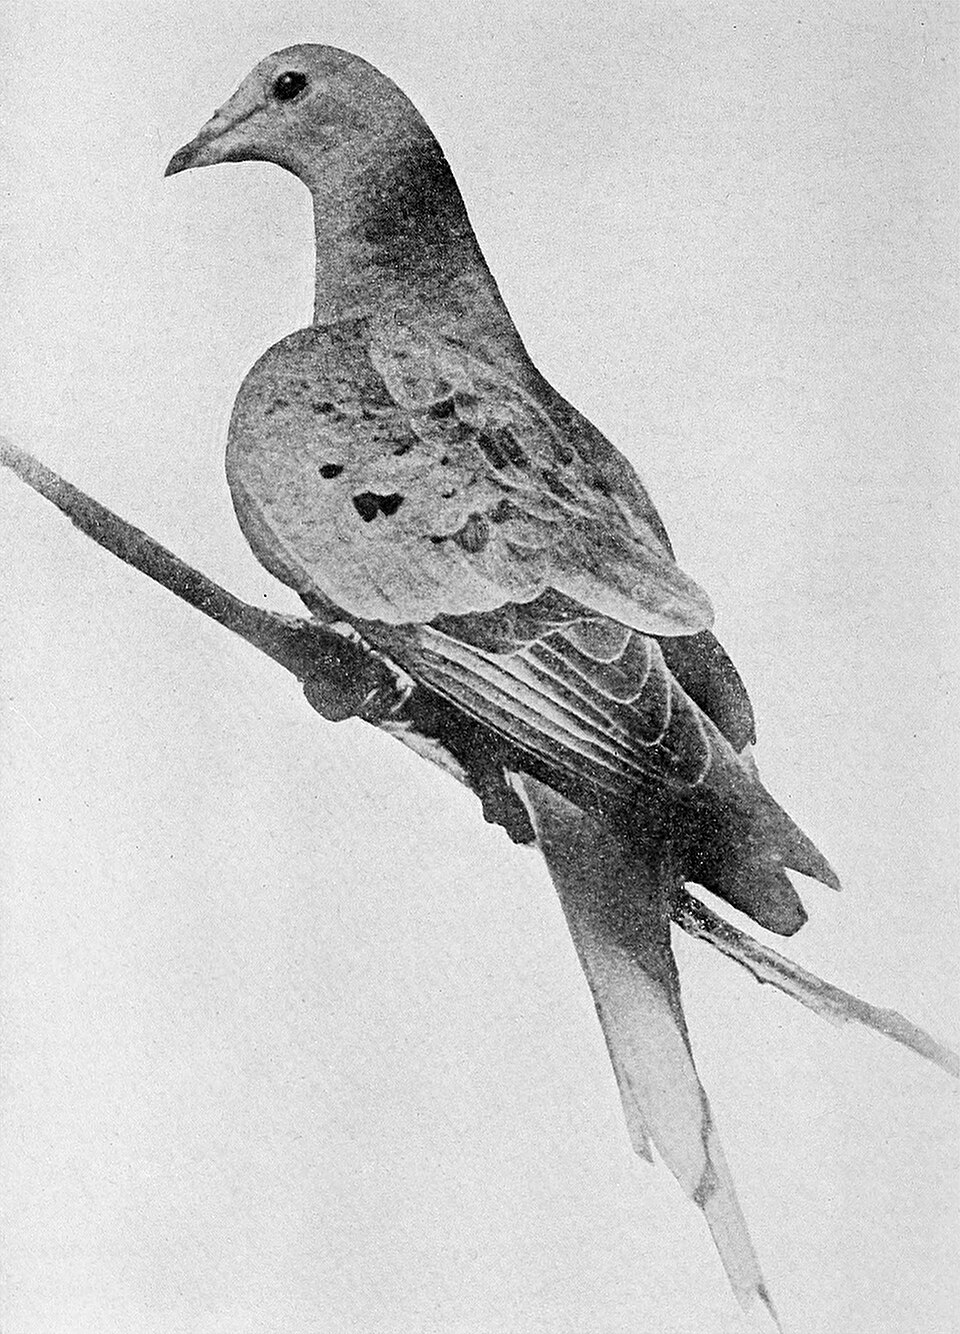
\includegraphics[width=0.4\linewidth]{images/book5/martha.jpg}\hspace{0.04\linewidth}
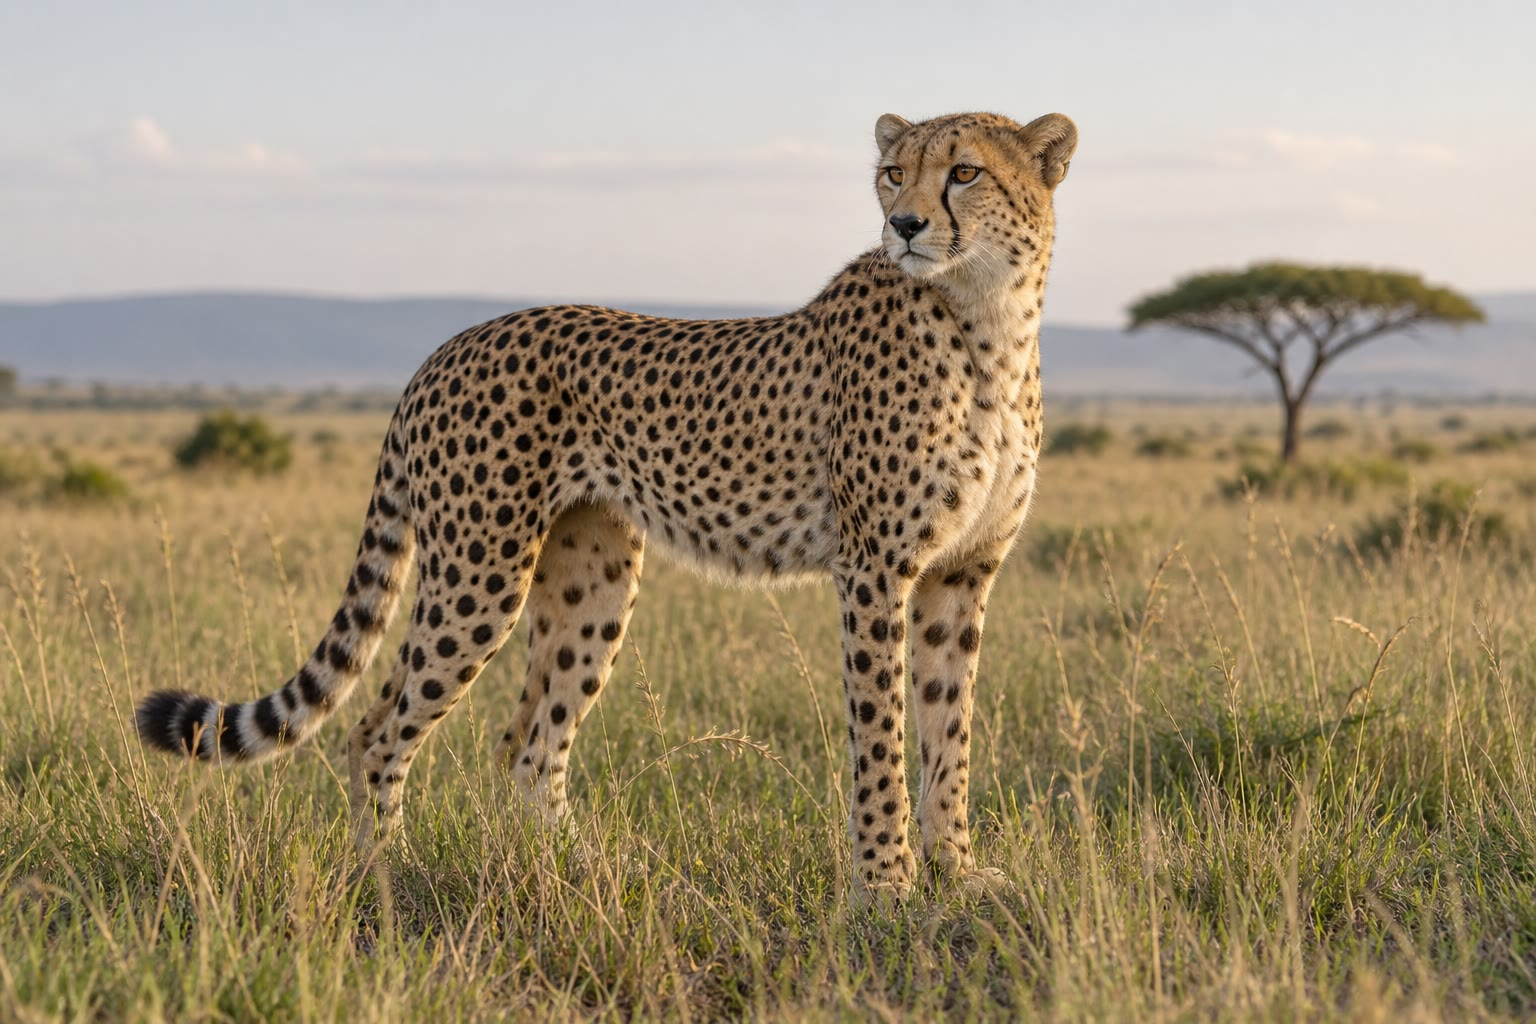
\includegraphics[width=0.52\linewidth]{images/book5/ai/b5-27-cheetah.jpg}

{\small Links: Martha, de laatste trekduif, in 1912 gefotografeerd in
de dierentuin van Cincinnati; de soort had binnen de herinnering van de
levenden nog miljarden geteld (foto door Enno Meyer, publiek domein).
Rechts: een cheeta --- een soort die zo'n tienduizend jaar geleden door
een flessenhals is gegaan en wier dieren zo sterk op elkaar lijken dat
huidtransplantaten tussen niet-verwante dieren niet worden afgestoten.}
\end{omfigure}

\section{Leefgebied: hoeveel, en in welke vorm}

\begin{proposition}[Soorten en oppervlakte]\label{prop:b3:conservation-biology:area}
\index{soort--oppervlakteverband}\index{versnippering van leefgebied}\index{eilandbiogeografie}\index{corridor}\index{SLOSS-debat}\index{randeffect}
Over eilanden, en over stukken leefgebied die zich als eilanden
gedragen, stijgt het aantal soorten $S$ met de oppervlakte $A$ als een
machtswet,
\[
S = c\,A^{z}, \qquad z \approx 0.15\text{--}0.35,
\]
het \emph{\omterm{prop:b3:conservation-biology:area}{soort--oppervlakteverband}} (Arrhenius, 1921; de
\omterm{prop:b3:conservation-biology:area}{eilandbiogeografie} van MacArthur en Wilson, 1967, verklaarde het als
een evenwicht tussen immigratie en uitsterven, waarbij het uitsterven
op kleine eilanden sneller gaat). Met $z = 0.25$ kost het verlies van
\qty{90}{\%} van de oppervlakte van een leefgebied uiteindelijk
$1 - 0.1^{0.25} = \qty{44}{\%}$ van zijn soorten; de helft verliezen
kost \qty{16}{\%}. Het verlies komt niet meteen --- een
\emph{uitstervingsschuld} wordt over decennia betaald terwijl
populaties die voor hun snipper te klein zijn wegkwijnen --- en de
\emph{versnippering} van een vaste oppervlakte in stukken brengt eigen
verliezen mee: elke snipper herbergt een kleinere populatie,
\emph{\omterm{prop:b3:conservation-biology:area}{randeffecten}} (wind, hitte, roofdieren, onkruid) dringen
honderden meters het bos in, en soorten die de binnenkant nodig hebben
verliezen meer dan de oppervlakte verklaart. Of één groot reservaat dan
wel verscheidene kleine met dezelfde totale oppervlakte meer soorten
redt (het \emph{SLOSS}-debat) hangt van de soorten af: het grote
herbergt grotere populaties en binnenkant, de kleine spreiden het
risico van een ramp en bemonsteren meer typen leefgebied.
\emph{Corridors} die snippers verbinden laten individuen en genen
ertussen bewegen en maken van geïsoleerde populaties een metapopulatie
waarvan de delen na een plaatselijke uitsterving opnieuw kunnen worden
bevolkt en van inteelt kunnen worden gered --- en daarom is het land
tussen de reservaten evenzeer een zorg geworden als de reservaten zelf.
\end{proposition}
\begin{proof}
De machtswet is empirisch, op log--logassen gefit aan archipels, meren,
bergtoppen en bosstukken over de hele wereld; de waarde van $z$ is
lager voor stukken van een vasteland (immigratie houdt soorten
aanwezig) en hoger voor echte eilanden. Het verhoudingsgewijze verlies
volgt rechtstreeks: $S'/S = (A'/A)^{z}$. Het mechanisme van de
\omterm{prop:b3:conservation-biology:area}{eilandbiogeografie} werd getoetst door Simberloff en Wilson (1969), die
kleine mangrove-eilandjes in Florida uitrookten en er elk geleedpotige
doodden, en die de aantallen soorten binnen een jaar naar hun vorige
waarden zagen terugkeren --- een evenwicht, met andere soorten dan
tevoren: het aantal wordt door oppervlakte en afstand bepaald, de
identiteiten door het toeval.
\end{proof}

\begin{omfigure}
\begin{tikzpicture}
\begin{loglogaxis}[
  width=0.6\linewidth, height=5.4cm,
  axis x line=bottom, axis y line=left,
  xmin=0.5, xmax=20000, ymin=5, ymax=300,
  xlabel={oppervlakte (km$^2$)}, ylabel={aantal soorten},
  xlabel style={font=\small, at={(axis description cs:0.5,-0.12)}, anchor=north}, ylabel style={font=\small},
  tick label style={font=\small}, xtick={1,10,100,1000,10000}, xticklabels={1,10,100,1000,10000}, ytick={10,30,100,300}, yticklabels={10,30,100,300},
  clip=false,
]
\addplot[very thick, omDef, domain=0.5:20000, samples=40] {20*x^0.25};
\addplot[only marks, mark=*, mark size=1.8pt, omDef!70!black] coordinates {(1,22) (3,24) (10,38) (30,44) (100,66) (300,80) (1000,110) (3000,150) (10000,190)};
\draw[dashed, gray] (axis cs:10000,5) -- (axis cs:10000,200) -- (axis cs:0.5,200);
\draw[dashed, gray] (axis cs:1000,5) -- (axis cs:1000,112.5) -- (axis cs:0.5,112.5);
\node[font=\scriptsize, omDef, anchor=south west] at (axis cs:1.2,215) {$S = c\,A^{0.25}$: helling $z$ op logassen};
\node[font=\scriptsize, anchor=west, align=left] at (axis cs:1200,40) {verlies \qty{90}{\%} van de oppervlakte:\\behoud $0.1^{0.25} = \qty{56}{\%}$\\van de soorten};
\end{loglogaxis}
\end{tikzpicture}

{\small De soort--oppervlaktewet op logaritmische assen. Haar helling
is de exponent $z$; daaruit is het uiteindelijke verlies aan soorten
uit een gekrompen leefgebied af te lezen --- een tiende van het bos
houdt ongeveer de helft van de soorten, en niet het tiende dat een
lineaire gok zou geven.}
\end{omfigure}

\begin{omfigure}
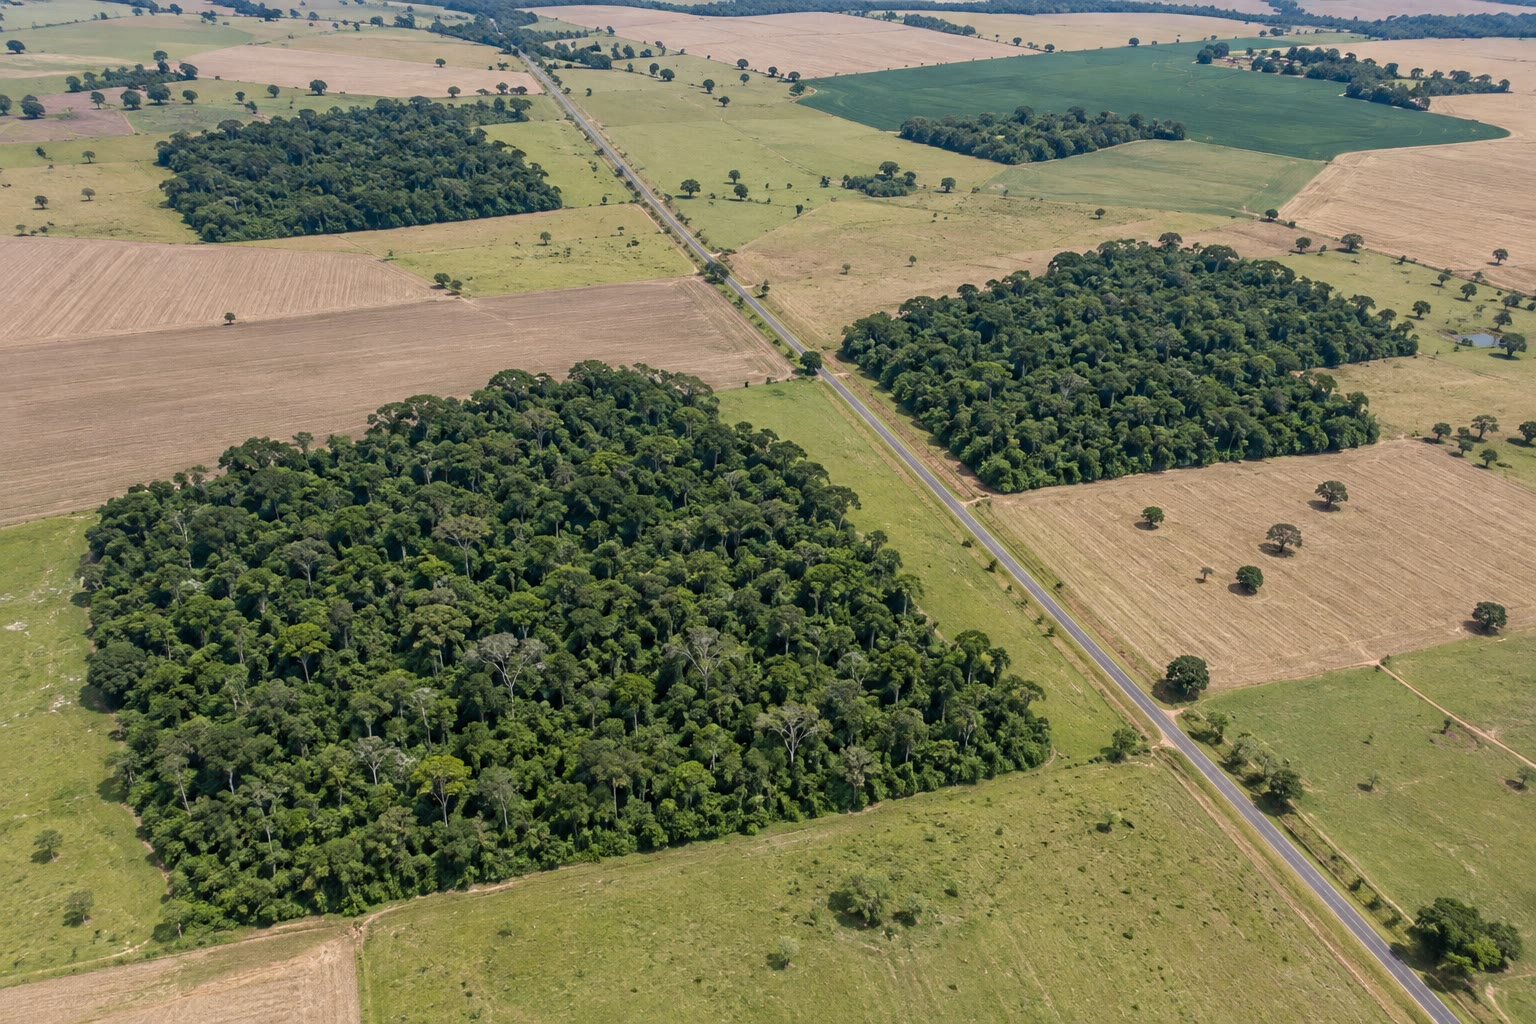
\includegraphics[width=0.6\linewidth]{images/book5/ai/b5-27-forest-fragments.jpg}

{\small Bossnippers in landbouwgrond, vanuit de lucht gezien: elk
eiland herbergt een kleinere populatie dan het geheel deed, is omzoomd
door een zone die de soorten van de binnenkant niet kunnen gebruiken,
en is gescheiden door akkers die de bossoorten niet kunnen oversteken.}
\end{omfigure}

\section{Voorspellen en voorkomen}

\begin{method}[Analyse van de levensvatbaarheid]\label{met:b3:conservation-biology:pva}
\index{analyse van de levensvatbaarheid}\index{quasi-uitsterving}
Om het uitstervingsrisico van een populatie te schatten en te zien wat
het zou verkleinen: (1) bouw een model van haar dynamiek --- een matrix
van overleving en vruchtbaarheid per leeftijd of per stadium, zoals in
de demografie van het deel van het tweede jaar, geschat uit gemerkte
dieren over enkele jaren; (2) voeg toevalligheid toe --- demografisch,
door het lot van elk individu te loten, en van de omgeving, door de
waarden van elk jaar uit hun waargenomen variantie te loten, met nu en
dan een ramp; (3) voeg dichtheidsafhankelijkheid en de genetische
achteruitgang door inteelt toe waar de gegevens dat toelaten;
(4) simuleer duizenden banen vanaf de huidige omvang over de gewenste
termijn en noteer het deel dat onder een drempel van
\emph{quasi-uitsterving} zakt (een omvang waarvandaan herstel onmogelijk
wordt geacht); (5) varieer de invoer --- de overleving van volwassenen,
die van jongen, de oppervlakte leefgebied, het overbrengen van tien
dieren --- en kijk welke verandering het risico het meest verkleint;
daar hoort de inspanning naartoe. De uitkomst is een kans met een grote
onzekerheid, geen voorspelling; haar waarde is vergelijkend, en zij
heeft herhaaldelijk laten zien dat bij langlevende soorten de
overleving van volwassenen en niet de vruchtbaarheid de hefboom is, en
daarom doden vislijnen populaties albatrossen die eens per twee jaar
één ei leggen sneller dan enig verlies van nesten zou kunnen.
\end{method}

\begin{proposition}[Tijd tot uitsterven]\label{prop:b3:conservation-biology:time}
\index{uitstervingstijd}
Voor een populatie die schommelt omdat de omgeving dat doet, met een
gemiddeld groeitempo $\bar r$ nabij nul en een variantie $\sigma^{2}$
in het jaarlijkse groeitempo, voert de logaritme van de
populatiegrootte een toevalswandeling met drift uit, en groeit de
verwachte tijd tot uitsterven vanaf omvang $N$ slechts als de
\emph{logaritme} van $N$ wanneer $\bar r < 0$ --- de populatie
verdubbelen voegt een vast aantal jaren toe --- en als een \emph{macht}
van $N$ wanneer $\bar r > 0$, met exponent $2\bar r/\sigma^{2} - 1$;
onder \omterm{def:b3:conservation-biology:small}{demografische toevalligheid} alleen groeit zij
\emph{exponentieel} met $N$, zodat een populatie die bij honderd veilig
is voor demografisch toeval bij tienduizend nog altijd aan de variantie
van de omgeving verloren kan gaan. Het praktische gevolg is dat het
verkleinen van de variantie van de groei van een populatie --- haar
tegen slechte jaren bufferen met meer leefgebied, meer plekken, een
breder dieet --- meer voor haar voortbestaan kan doen dan het verhogen
van haar gemiddelde.
\end{proposition}
\admitted

\begin{omfigure}
\begin{tikzpicture}
\begin{semilogyaxis}[
  width=0.62\linewidth, height=5.4cm,
  axis x line=bottom, axis y line=left,
  xmin=0, xmax=50, ymin=1, ymax=3000,
  xlabel={jaren}, ylabel={populatiegrootte},
  xlabel style={font=\small, at={(axis description cs:0.5,-0.12)}, anchor=north}, ylabel style={font=\small},
  tick label style={font=\small}, xtick={0,10,20,30,40,50}, ytick={1,10,100,1000}, yticklabels={1,10,100,1000},
  clip=false,
]
\addplot[thick, omDef] coordinates {(0,200) (2,240) (4,190) (6,260) (8,300) (10,220) (12,180) (14,250) (16,330) (18,280) (20,350) (22,300) (24,260) (26,340) (28,420) (30,380) (32,450) (34,400) (36,520) (38,480) (40,560) (42,500) (44,600) (46,650) (48,610) (50,700)};
\addplot[thick, omThm] coordinates {(0,200) (2,150) (4,180) (6,120) (8,90) (10,110) (12,70) (14,50) (16,60) (18,35) (20,40) (22,25) (24,18) (26,22) (28,12) (30,8) (32,9) (34,5) (36,3) (38,2) (40,1)};
\addplot[thick, omMeth!70!black] coordinates {(0,200) (2,210) (4,170) (6,200) (8,140) (10,160) (12,120) (14,140) (16,90) (18,110) (20,80) (22,95) (24,60) (26,75) (28,50) (30,55) (32,40) (34,45) (36,30) (38,35) (40,28) (42,30) (44,22) (46,25) (48,20) (50,22)};
\draw[dashed, gray] (axis cs:0,20) -- (axis cs:50,20); \node[font=\scriptsize, gray, anchor=north east] at (axis cs:49,18) {drempel van quasi-uitsterving};
\node[font=\scriptsize, omDef, anchor=west] at (axis cs:50.5,700) {$\bar r > 0$: houdt stand};
\node[font=\scriptsize, omMeth!70!black, anchor=west] at (axis cs:50.5,22) {$\bar r \approx 0$: zakt af};
\node[font=\scriptsize, omThm, anchor=west] at (axis cs:40.5,1.3) {$\bar r < 0$: weg in 40 jaar};
\end{semilogyaxis}
\end{tikzpicture}

{\small Drie gesimuleerde banen vanaf dezelfde tweehonderd dieren, die
alleen in hun gemiddelde groeitempo verschillen; een \omterm{met:b3:conservation-biology:pva}{analyse van de
levensvatbaarheid} laat er duizenden lopen en telt hoeveel er de drempel
overschrijden. De variantie van jaar tot jaar is wat zelfs het
middelste geval tot een gok maakt.}
\end{omfigure}

\begin{definition}[Het gereedschap]\label{def:b3:conservation-biology:tools}
\index{Rode Lijst van de IUCN}\index{invasieve soort}\index{ex-situbehoud}\index{fokken in gevangenschap}\index{herintroductie}\index{verwildering}\index{trofische cascade}
De \emph{Rode Lijst van de IUCN} deelt soorten in naar kwantitatieve
maatstaven: een achteruitgang van \qty{30}{\%}, \qty{50}{\%} of
\qty{80}{\%} over tien jaar of drie generaties, een
verspreidingsgebied onder \qty{20000}{}, \qty{5000}{} of
\qty{100}{km^2}, een populatie onder \qty{10000}{}, \qty{2500}{} of
\qty{250}{} volwassen dieren, of een berekende uitstervingskans,
plaatsen een soort als Kwetsbaar, Bedreigd of Ernstig Bedreigd; een
kwart van de zoogdieren en een achtste van de vogels komt in
aanmerking. De oorzaken zijn in de eerste plaats het verlies van
leefgebied, dan overbejaging, \emph{invasieve soorten} (roofdieren en
concurrenten die naar eilanden zijn gebracht wier soorten hen nooit
hadden ontmoet: ratten, katten en hermelijnen hebben de meeste vogels
van Nieuw-Zeeland genomen, één soort bruine boomslang de meeste van
Guam), vervuiling en klimaatverandering. De antwoorden: beschermde
gebieden die een zesde van het land beslaan; het beheersen of uitroeien
van indringers (honderdvijftig eilanden zijn van ratten ontdaan); het
\emph{ex-situ}-behoud --- zaadbanken met een miljoen monsters in een
kluis in de arctische permafrost, ingevroren embryo's, en het
\emph{fokken in gevangenschap} met stambomen die zo worden beheerd dat
de verwantschap zo klein mogelijk blijft, wat de Californische condor
van tweeëntwintig vogels in 1987 en de zwartvoetbunzing van achttien
heeft teruggebracht; de \emph{herintroductie}, die ongeveer een derde
van de keren slaagt en vaker wanneer de oorzaak van het oorspronkelijke
verlies is weggenomen; en de \emph{verwildering}, de terugkeer van
grote dieren en van de processen die zij aandrijven --- de wolven van
Yellowstone, wier predatie en de vrees ervoor de wapiti's van de
rivieroevers verdreven en wilg, esp, bever en zangvogels lieten
terugkeren, een \emph{trofische cascade} die van een roofdier tot de
vorm van een rivier loopt.
\end{definition}

\begin{omfigure}
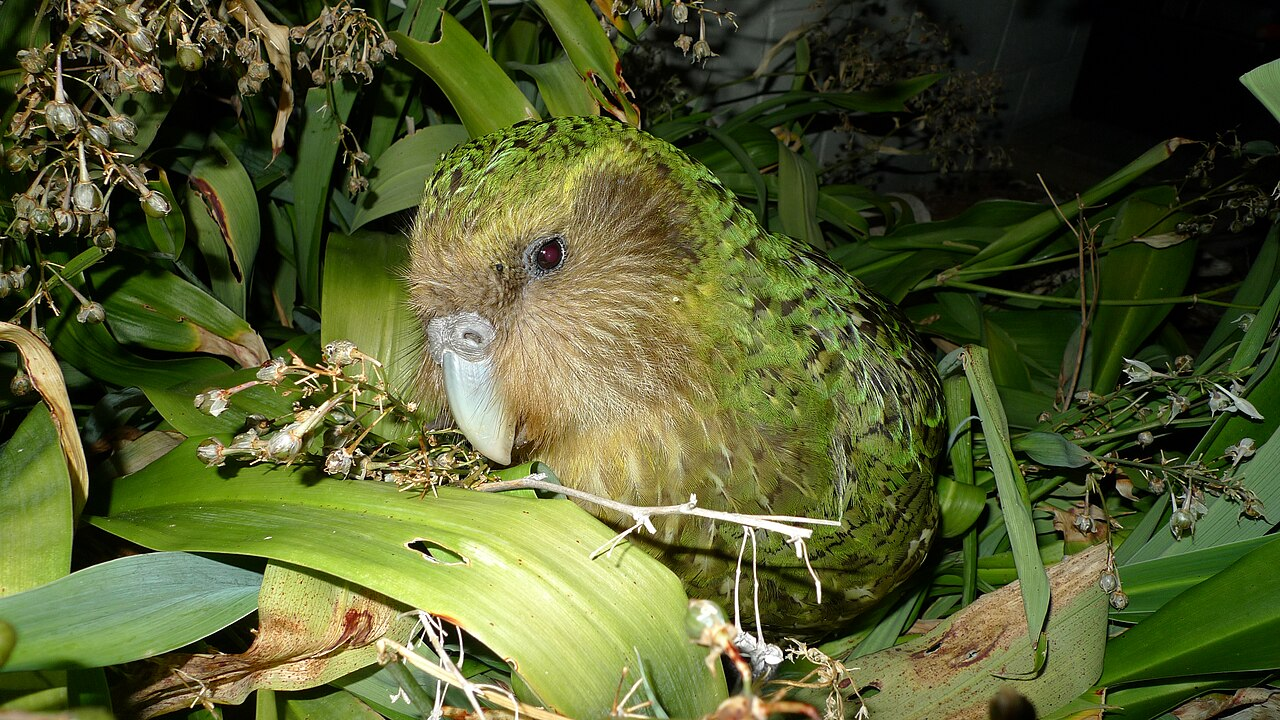
\includegraphics[width=0.46\linewidth]{images/book5/kakapo-sirocco.jpg}\hspace{0.04\linewidth}
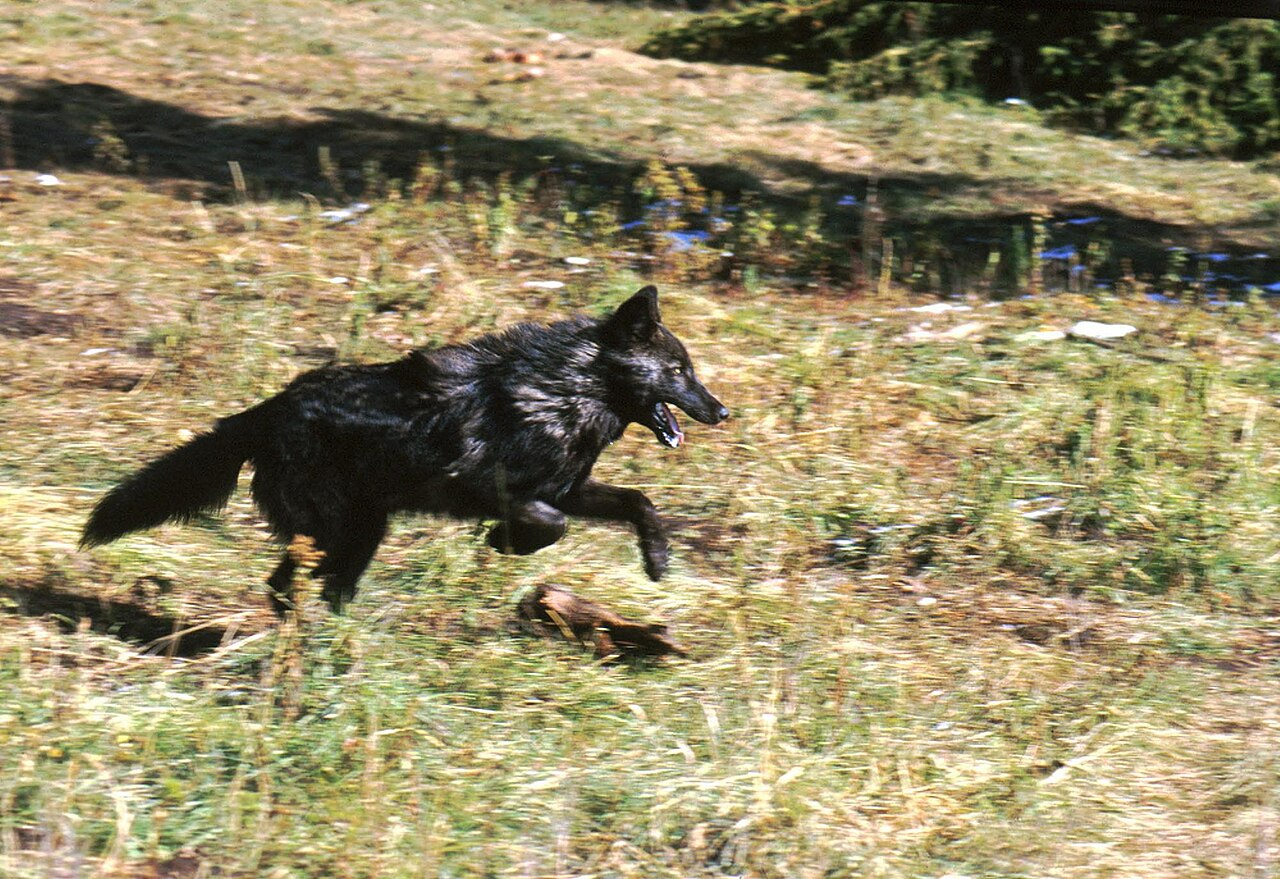
\includegraphics[width=0.46\linewidth]{images/book5/yellowstone-wolves-1996.jpg}

{\small Links: Sirocco, een kakapo --- een van de eenenvijftig
overlevenden in 1995, nu een van zo'n tweehonderdvijftig, elk met een
naam en gevolgd op eilanden zonder roofdieren (foto: Department of
Conservation, Nieuw-Zeeland, CC BY 2.0). Rechts: wolven in Yellowstone
in 1996, de eerste winter na hun \omterm{def:b3:conservation-biology:tools}{herintroductie} (foto: National Park
Service, publiek domein).}
\end{omfigure}

\begin{example}[Drie herstelverhalen]\label{ex:b3:conservation-biology:recoveries}
De kakapo: eenenvijftig vogels in 1995, alle overgebracht naar eilanden
die van roofdieren waren ontdaan; elke vogel draagt een zender, elk
nest wordt met een camera bewaakt, kuikens worden met de hand
grootgebracht wanneer een moeder faalt, mannetjes worden bijgevoerd om
hen in broedconditie te brengen in de jaren waarin de rimubomen vrucht
dragen, en de stamboom wordt zo beheerd dat de zeldzame genen van het
laatste mannetje uit Fiordland in de populatie blijven; van elke kakapo
is het genoom bepaald. Tweehonderdvijftig nu, en een $N_{e}$ die de
genomen nabij honderd leggen. De trompetkraanvogel: vijftien vogels in
1941, één trekkende zwerm, in gevangenschap gefokt uit eieren die uit
wilde nesten waren gehaald, nieuwe trekroutes geleerd achter
ultralichte vliegtuigen aan, en nu zo'n achthonderd. De bultrug: tot
een paar duizend bejaagd, in 1966 beschermd, en voorbij de
honderdduizend, een toename van bijna \qty{8}{\%} per jaar die laat
zien wat een langlevend dier doet wanneer de enige oorzaak van zijn
achteruitgang wordt weggenomen. Elk herstel kostte tientallen miljoenen
en decennia; de rekenkunde van dit hoofdstuk zegt waarom de inspanning
moest worden geleverd voordat de aantallen de draaikolk bereikten, en
waarom zij goedkoper was dan elke latere redding zou zijn geweest.
\end{example}

\begin{omfigure}
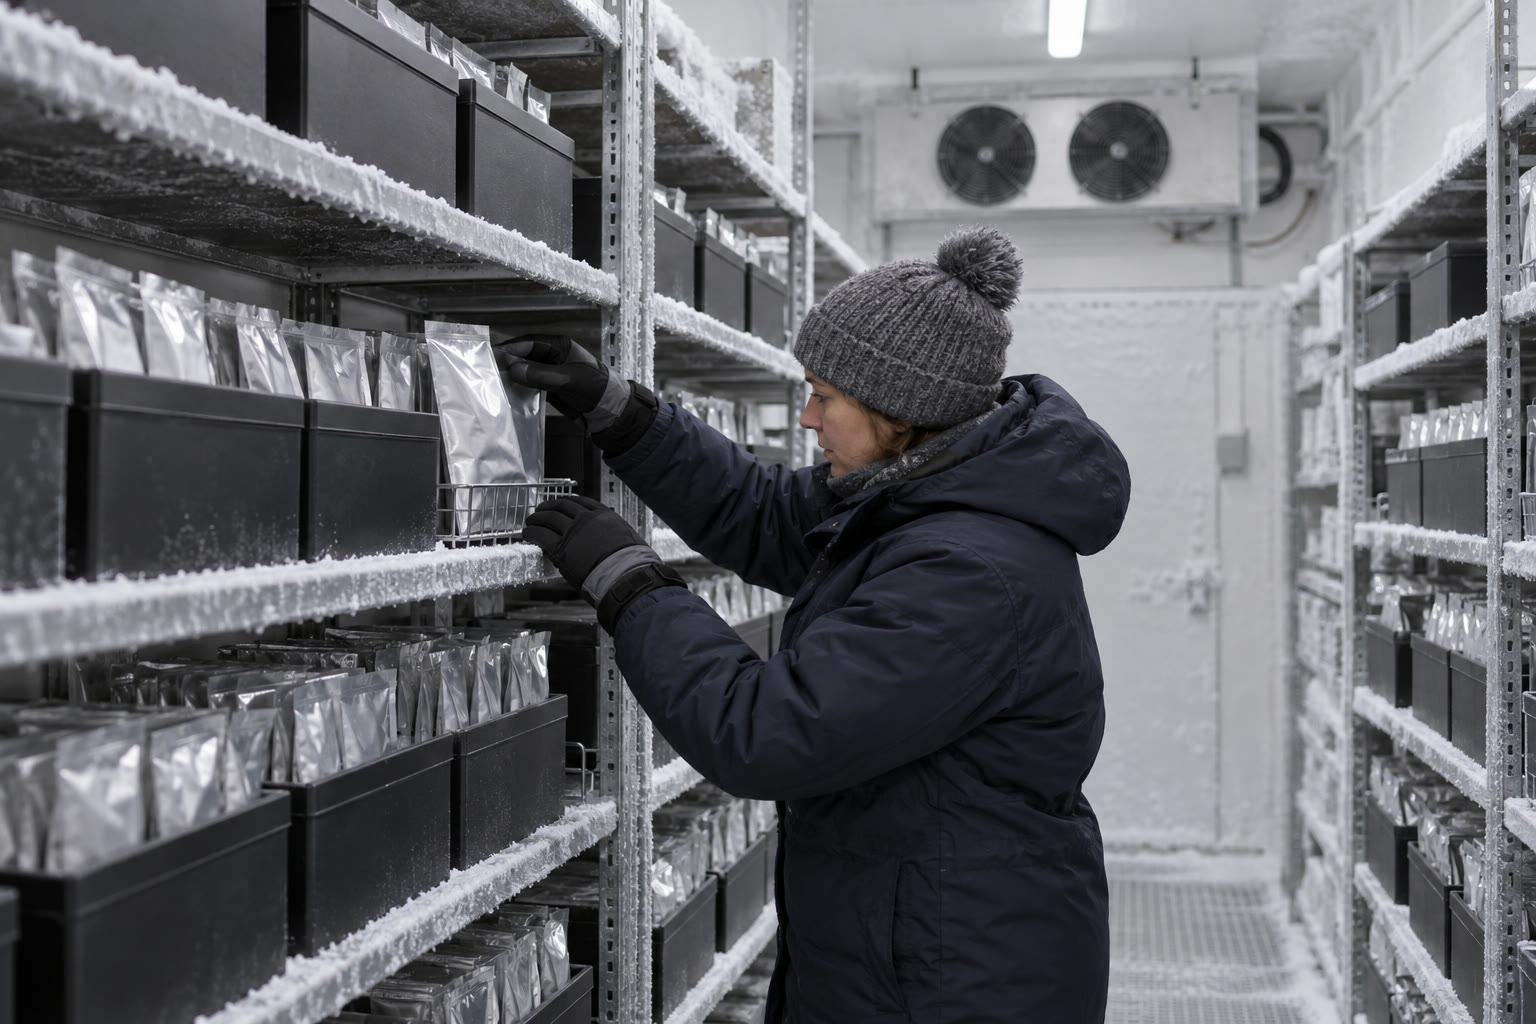
\includegraphics[width=0.56\linewidth]{images/book5/ai/b5-27-seed-vault.jpg}

{\small Een zaadkluis in de permafrost: duplicaten van een miljoen
monsters van gewassen en wilde planten, bij \qty{-18}{\celsius} bewaard
tegen het verlies van de verzamelingen waaruit zij komen ---
natuurbehoud als verzekering, op de schaal van het genoom van een soort.}
\end{omfigure}

\begin{remark}[De rekenkunde van het behouden]\label{rem:b3:conservation-biology:remark}
Elk hoofdstuk van deze cursus is in een getal geëindigd, en dit eindigt
in verscheidene: een effectieve grootte, een \omterm{thm:b3:conservation-biology:ne}{inteeltcoëfficiënt} die per
generatie met $1/2N_{e}$ stijgt, een exponent $z$ die verloren hectaren
in verloren soorten omzet, een kans op uitsterven in een eeuw. Zij zijn
grof --- de telling is onzeker, de variantie is geraden, het model is
een karikatuur --- en zij zijn wat een gevoel over verdwijnende vogels
omzet in een beslissing over welke vijftig hectare te kopen en welke
acht dieren te verplaatsen. De biologie is dezelfde biologie als in de
rest van het boek: drift, selectie, demografie, gedrag, de
afhankelijkheid van een populatie van haar leefgebied en van een
leefgebied van zijn populaties. Nieuw is alleen de urgentie, en het
feit dat het experiment één keer wordt uitgevoerd, zonder controle, op
de soorten die er nog zijn.
\end{remark}

\section{Opgaven}

\begin{exercise}[$\star$]\label{exo:b3:conservation-biology:1}
Definieer de \omterm{def:b3:conservation-biology:small}{demografische toevalligheid}, de \omterm{def:b3:conservation-biology:small}{toevalligheid van de
omgeving} en het \omterm{def:b3:conservation-biology:small}{Allee-effect}, en geef van elk een voorbeeld uit dit
hoofdstuk.
\end{exercise}

\begin{exercise}[$\star$]\label{exo:b3:conservation-biology:2}
Wat is de \omterm{thm:b3:conservation-biology:ne}{effectieve populatiegrootte}, en noem drie kenmerken van een
echte populatie die haar kleiner maken dan de telling.
\end{exercise}

\begin{exercise}[$\star$]\label{exo:b3:conservation-biology:3}
Formuleer de soort--oppervlaktewet. Welk deel van de soorten houdt een
leefgebied bij $z = 0.25$ over nadat het de helft van zijn oppervlakte
heeft verloren? En negen tiende? En negenennegentig honderdste?
\end{exercise}

\begin{exercise}[$\star$]\label{exo:b3:conservation-biology:4}
Leg de regel 50/500 uit, en waartegen elk van beide getallen beschermt.
\end{exercise}

\begin{exercise}[$\star\star$]\label{exo:b3:conservation-biology:5}
Een kudde van 200 zeeolifanten heeft 8 broedende mannetjes en 120
broedende vrouwtjes. Bereken $N_{e}$ en het verlies aan heterozygotie
per generatie. Hoeveel generaties om er een kwart van te verliezen?
\end{exercise}

\begin{exercise}[$\star\star$]\label{exo:b3:conservation-biology:6}
Een populatie telde in vijf opeenvolgende generaties 1000, 1000, 20,
1000, 1000. Bereken $N_{e}$ over dat bestek, en de behouden
heterozygotie, en vergelijk met een constante 1000.
\end{exercise}

\begin{exercise}[$\star\star$]\label{exo:b3:conservation-biology:7}
Vijfentwintig Florida-panters met $N_{e} \approx 10$: hoeveel inteelt
is er in 5 generaties opgebouwd? Als de fitness met \qty{5}{\%} daalt
voor elke \qty{10}{\%} van $F$, hoeveel is de fitness dan gedaald? Wat
doet het toevoegen van acht niet-verwante vrouwtjes met $F$ in de
volgende generatie?
\end{exercise}

\begin{exercise}[$\star\star$]\label{exo:b3:conservation-biology:8}
Yellowstone: in 1995--96 zijn er 31 wolven uitgezet, en in 2003 waren
er ongeveer 100 in het park. Schat $r$; hoeveel zouden er in 2020 zijn
geweest als de groei had aangehouden, en waarom is dat niet gebeurd?
\end{exercise}

\begin{exercise}[$\star\star$]\label{exo:b3:conservation-biology:9}
Deel in volgens de IUCN-maatstaven uit dit hoofdstuk: (a) een kikker
wier populatie in tien jaar \qty{60}{\%} is gedaald; (b) een plant met
180 volwassen exemplaren; (c) een vis wier verspreidingsgebied
\qty{3000}{km^2} is; (d) een vogel met \num{30000} exemplaren die per
decennium \qty{10}{\%} achteruitgaat.
\end{exercise}

\begin{exercise}[$\star\star\star$]\label{exo:b3:conservation-biology:10}
Een populatie van $N$ paren die elk met kans $1/2$ twee overlevende
nakomelingen voortbrengen en anders geen (\omterm{def:b3:conservation-biology:small}{demografische toevalligheid}).
Bereken de kans dat de hele populatie in één generatie faalt voor
$N = 2$, $5$, $10$ en $20$, en geef commentaar op hoe het demografische
risico met $N$ schaalt.
\end{exercise}

\begin{exercise}[$\star\star\star$]\label{exo:b3:conservation-biology:11}
De soort--oppervlaktewet met $z = 0.25$, en een bos dat in 10 gelijke
geïsoleerde snippers is gesneden. Vergelijk het aantal soorten dat in
één snipper wordt verwacht met een tiende van het oorspronkelijke
aantal, en beredeneer waarom het totaal over de snippers niet
eenvoudig het oorspronkelijke is --- wat bepaalt of de snippers samen
meer of minder soorten herbergen dan het geheel deed?
\end{exercise}

\begin{exercise}[$\star\star\star$]\label{exo:b3:conservation-biology:12}
Waarom stopt het toevoegen van een paar migranten per generatie
($m N_{e} \approx 1$) het verlies aan variatie in een kleine populatie
grotendeels, en wat kost dat aan plaatselijke aanpassing? Gebruik het
evenwicht tussen de drift, $1/2N_{e}$, en het deel van de allelen dat
door migranten wordt vervangen, $m$, om te beredeneren.
\end{exercise}

\section{Vraagstuk: vijftig en vijfhonderd}

\begin{problem}[{Weekendvraagstuk --- een herstelprogramma in getallen:
de effectieve grootte van een geredde papegaaienpopulatie en haar
inteelt, een genetische redding, de soorten die een krimpend bos zal
behouden, de groei van uitgezette wolven, en de categorieën en de
kosten, eindigend bij $N_{e}$, de inteelt na tien generaties en het
deel van de soorten dat behouden blijft}]
\label{pb:b3:conservation-biology:1}
Gegevens: een papegaaienpopulatie van 60 volwassen dieren, 20 mannetjes
en 40 vrouwtjes, die alle broeden; generatieduur \qty{10}{yr}. De
geschiedenis van de populatie over de laatste vijf generaties: 500,
100, 60, 51, 60. Inteeltdepressie: de fitness daalt met \qty{6}{\%} per
\qty{0.1}{} van $F$. Redding: 10 niet-verwante vogels toegevoegd aan de
60. Bos: \qty{2000}{km^2} teruggebracht tot \qty{300}{km^2}, $z = 0.25$;
nu 180 soorten. Wolven: 31 uitgezet, 100 na 8 jaar, draagkracht in het
park ongeveer 120. Kosten: vier miljoen dollar per jaar voor de
papegaaien.

\medskip
\noindent\textbf{Deel I --- Effectieve grootte.}
\begin{enumerate}
  \item $N_{e}$ uit de \omterm{thm:b3:conservation-biology:ne}{geslachtsverhouding} van de huidige 60. Vergelijk
        met de telling.
  \item Het \omterm{thm:b3:conservation-biology:ne}{harmonisch gemiddelde} $N_{e}$ over de vijf generaties
        geschiedenis. Welke generatie overheerst?
  \item De inteelt die over die vijf generaties is opgebouwd, met het
        \omterm{thm:b3:conservation-biology:ne}{harmonisch gemiddelde} $N_{e}$ (exacte formule en lineaire benadering).
  \item De fitness die aan die inteelt verloren gaat.
  \item De heterozygotie die na de vijf generaties resteert, als
        fractie van de oorspronkelijke.
  \item Als de populatie nu op 60 wordt gehouden met de huidige
        \omterm{thm:b3:conservation-biology:ne}{geslachtsverhouding}, welke $F$ bereikt zij dan in tien
        generaties meer, en welk verlies aan fitness? Hoeveel jaar is dat?
\end{enumerate}

\medskip
\noindent\textbf{Deel II --- Redding.}
\begin{enumerate}[resume]
  \item Tien niet-verwante vogels voegen zich bij de 60. Het deel van
        de allelen in de volgende generatie dat van de nieuwkomers komt
        is ongeveer $10/70$; de \omterm{thm:b3:conservation-biology:ne}{inteeltcoëfficiënt} van nakomelingen met
        één inheemse en één nieuwe ouder is $0$. Schat de gemiddelde
        $F$ van de populatie in de volgende generatie bij willekeurige
        paring.
  \item Leg uit waarom $F$ meteen daalt maar de heterozygotie pas
        stijgt naarmate de allelen van de migranten zich verspreiden,
        en waarom er een tweede redding nodig kan zijn.
  \item Hoeveel volwassen dieren zijn er nodig om $N_{e} = 500$ te
        bereiken bij een gelijke \omterm{thm:b3:conservation-biology:ne}{geslachtsverhouding}? Hoeveel jaar bij
        $r = \qty{0.05}{yr^{-1}}$ vanaf 70 vogels?
  \item Het programma haalt eieren weg bij zwakke moeders om ze met de
        hand groot te brengen, wat het gemiddelde aantal uitgevlogen
        jongen per paar verhoogt maar de gezinsgrootten gelijkmaakt.
        Waarom \emph{verhoogt} het gelijkmaken van de gezinsgrootten
        $N_{e}$ boven de telling (naar $2N$)?
  \item Het laatste mannetje van een aparte zuidelijke lijn is in het
        wild onvruchtbaar. Stel twee ingrepen voor en hun kosten voor de
        genenpoel.
  \item Bij vier miljoen dollar per jaar over de 40 jaar tot
        $N_{e} = 500$: de totale kosten, en de kosten per extra vogel. Is dat duur?
        Waartegen afgezet?
\end{enumerate}

\medskip
\noindent\textbf{Deel III --- Het bos.}
\begin{enumerate}[resume]
  \item Het deel van de soorten dat het bos bij \qty{300}{km^2} zal
        behouden; het verwachte aantal soorten, en de uitstervingsschuld
        (de soorten die er nu zijn en die zullen verdwijnen).
  \item Als de \qty{300}{km^2} in plaats daarvan drie geïsoleerde
        snippers van \qty{100}{km^2} waren: het aantal soorten per
        snipper; het totaal als de snippers geheel verschillende
        soorten herbergden; het totaal als zij dezelfde herbergden. Wat
        beslist dat?
  \item Een corridor van \qty{20}{km^2} verbindt de drie snippers.
        Behandel ze als één gebied van \qty{320}{km^2}: het verwachte
        aantal soorten. Vergelijk met het geval van gelijke soorten uit
        vraag~14.
  \item Het grootste roofdier van het bos heeft \qty{50}{km^2} per paar
        nodig en een $N_{e}$ van 50 om stand te houden. Kan de hele
        \qty{300}{km^2} het herbergen? Kan een snipper dat? Wat zegt dit
        over oppervlakte tegenover aantal soorten als maatstaf?
  \item Schat hoe lang het duurt voordat de uitstervingsschuld is
        betaald als de soorten die verloren gaan populaties hebben die
        met \qty{3}{\%} per jaar teruglopen van 200 tot een drempel van 10.
  \item Waarom onderschat de soort--oppervlaktewet het verlies wanneer
        de versnippering \omterm{prop:b3:conservation-biology:area}{randeffecten} toevoegt, en overschat zij het
        wanneer het omringende land deels bruikbaar is?
\end{enumerate}

\medskip
\noindent\textbf{Deel IV --- Wolven en lijsten.}
\begin{enumerate}[resume]
  \item Wolven: $r$ uit $31 \to 100$ in 8 jaar, en de verdubbelingstijd.
  \item Logistische groei naar $K = 120$: de populatie na 8 jaar bij
        logistische in plaats van exponentiële groei, uitgaande van 31
        met de $r$ van vraag~19 (gebruik $N(t) = K/[1 + (K/N_{0} -
        1)\mathrm{e}^{-rt}]$). Welke past beter bij de waargenomen 100,
        en wat zegt dat over de dichtheidsafhankelijkheid in de eerste
        jaren?
  \item De wapiti's telden \num{17000} in 1995 en \num{4000} in 2015.
        Het gemiddelde jaarlijkse tempo van achteruitgang. Hoeveel
        daarvan verklaren wolven die elk \num{20} wapiti's per jaar
        eten, bij 100 wolven?
  \item Deel de papegaai (60 volwassen exemplaren) en het roofdier van
        het bos van vóór de redding in volgens de IUCN-maatstaven.
  \item De trekduif: vijf miljard in 1800, uitgestorven in 1914. Als de
        achteruitgang exponentieel verliep vanaf 1870, toen er nog
        miljarden waren, tot één vogel in 1914, welk jaarlijks tempo
        betekent dat? Waarom maakt het \omterm{def:b3:conservation-biology:small}{Allee-effect} de laatste decennia
        sneller dan exponentieel?
  \item Leg in een alinea uit waarom een \omterm{met:b3:conservation-biology:pva}{analyse van de
        levensvatbaarheid} in 1850 zou hebben gezegd dat de trekduif
        veilig was, en wat zij over het hoofd zou hebben gezien.
  \item Vat samen: de huidige $N_{e}$ (vraag~1), $F$ na tien generaties
        meer bij 60 (vraag~6), en het deel van de soorten dat het
        gekrompen bos behoudt (vraag~13).
\end{enumerate}
\end{problem}
